\chapter{Observational Health Data Sciences and Informatics (OHDSI)}\label{cap:05OHDSI}

Este capítulo presenta el marco teórico sobre OHDSI y se divide en cinco secciones:  \ref{sec:05intro} Introducción, \ref{sec:05OHDSI} ¿Qué es OHDSI?, \ref{sec:05omop} ¿Qué es OMOP? \ref{sec:05Evidencia} ¿Cómo generar evidencia? y \ref{sec:05conclusion} Conclusión.

\section{Introducción} \label{sec:05intro}
%El objetivo es dar a concoer todos los conceptos teóricos de OHDSI y ATLAS. Quién quiera utilizar ATLAS debe conocer OHDSI, debe conocer el CDM, el Vocab, otras herramientas... Son conceptos fundamentales.

La organización Observational Health Data Science and Informatics (OHDSI) es muy importante para el TFG porque es la organización proveedora de la herramienta de análisis ATLAS, núcleo central del trabajo, y por la relevancia que ha adquirido a nivel europeo en los últimos años.

En este capítulo se da a conocer la organización y se identifican los conceptos, ideas y valores fundamentales de la misma. \textbf{Es necesario conocer OHDSI para comprender el proyecto en su totalidad y de forma profunda.} Además, satisface el Obj-002 del proyecto (véase \ref{sec:02objTFG} ''Objetivos del TFG'').

A continuación, en la sección \ref{sec:05OHDSI} ''¿Qué es OHDSI?'' se presenta lu visión, misión y valores de la organización y una serie de características fundamentales que la definen. 

En la sección \ref{sec:05omop} ''¿Qué es OMOP?'' se presenta  OMOP, la organización predecesora de OHDSI 
y creadora del conocido \textit{Modelo Común de Datos (CDM)}.

Por último, en la sección \ref{sec:05Evidencia} ''¿Cómo generar evidencia?'' se presenta la metodología común que promueve la organización para alcanzar la finalidad principal de generar evidencia a partir de datos observacionales. Es muy importante conocer estos conceptos a la hora de conducir un estudio utilizando herramientas OHDSI.

\section{¿Qué es OHDSI?} \label{sec:05OHDSI}

OHDSI, pronunciado en inglés ''Odyseey'', son las siglas de \textbf{Observational Health Data Science and Informatics}. El Libro de OHDSI \cite{OHDSIbook} define la organización como ''una comunidad de ciencia abierta que tiene como objetivo mejorar la salud empoderando a la comunidad para generar de manera colaborativa evidencia que promueva mejores decisiones de salud y mejor atención''. En la Figura \ref{fig:OHDSIbanner} ''Banner de OHDSI'' se muestra el logo de la organización.

\begin{figure}[H]
    \centering
    
\includegraphics[width=0.80\textwidth]{figures/OHDSIbanner.png}
    \caption{Banner de OHDSI. Extraído de web oficial \cite{OHDSIwebsite}}
    \label{fig:OHDSIbanner}
\end{figure}

La \textbf{misión} de la comunidad consiste en ''mejorar la salud empoderando a una comunidad para generar de manera colaborativa evidencia que promueva mejores decisiones de salud y una mejor atención'', y la \textbf{visión} consiste en ''un mundo en el que la investigación observacional produzca una comprensión integral de la salud y la enfermedad'' \cite{OHDSIwebsite}\cite{OHDSIbook}. 

La organización nació en 2014, como continuación del concluido proyecto OMOP (veáse a continuación \ref{sec:05omop} ''¿Qué es OMOP?'') y en la actualidad, cuenta con la participación de más de tres mil colaboradores distribuidos globalmente en 80 países.

\begin{figure}[H]
    \centering
    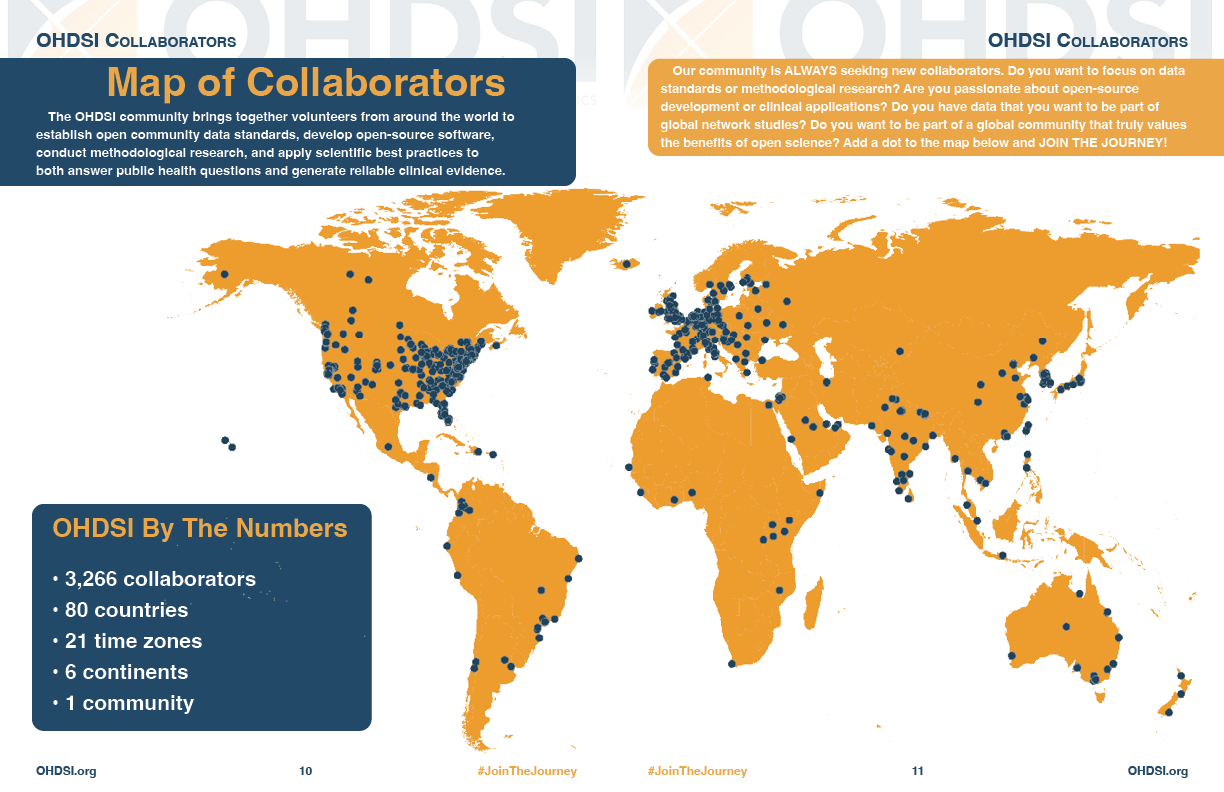
\includegraphics[width=0.80\textwidth]{figures/OHDSIcollaborators.png}
     \caption{Mapa de colaboradores de OHDSI. Extraído de la web oficial \cite{OHDSIwebsite}}
    \label{fig:OHDSIcollaborators}
\end{figure}

Haciendo referencia a la Figura \ref{fig:OHDSIcollaborators} ''Mapa de colaboradores de OHDSI'', la presencia en Europa de la organización es innegable. Desde que inició en 2020 su colaboración con la red europea de datos EHDEN \textit{(European Health Data Evidence)}, está adquiriendo cada vez mayor relevancia. Ejemplo de ello es la celebración este mes de junio en Rotterdam del quinto Symposium Europeo de OHDSI, con el fin de reunir a los expertos y miembros de la comunidad para presentar los grandes proyectos nacionales y europeos que se están realizando en toda europa con las herramientas de la comunidad.

%\begin{figure}[H]
%    \centering
%    
\includegraphics[width=0.70\textwidth]{figures/bannerSymposyum2024.jpg}
%     \caption{Banner del Symposium Europeo 2024. Extraído de la web oficial \cite{OHDSIwebsite}}
%    \label{fig:bannerSymposyum2024}
%\end{figure}

%Por ejemplo, en el Symposium Europeo del pasado año 2023, se presentaron proyectos relativos al almacenamiento de los datos de UCI en Holanda \cite{Jagesar2023The}, la integración del CDM de OMOP con el laboratorio de datos de salud alemám \cite{Finster2023Integrating}, la estandarización de la base de datos nacional francesa SNDS al modelo de OMOP \cite{Collumeau2023Standardization}, la armonización de los HCE hospitalarios en Ruanda al CDM \cite{Halvorsen2023Ruanda} y a la estandarización de los datos del registro europeo de sarcomas a OMOP \cite{vanSwieten2023Standardizing}, entre otros.

\subsection{Características de la organización} \label{subsec:05caracteristicas}

Más allá de los aspectos técnicos de la organización, en esta sección se presentan cuatro características inferidas de la investigación sobre OHDSI, que proveen una visión compresiva de la misma. De esta forma, OHDSI se caracteriza por ser: (i) una comunidad o red colaborativa, (ii) de ciencia abierta, (iii) que promueve la estandarización en salud y (iv) la extracción de evidencia a partir de datos clínicos.

\begin{itemize}

    \item \textbf{Una comunidad o red colaborativa}. La organización es una comunidad abierta a la incorporación de cualquiera que esté comprometido con su misión y valores. Este interés en la incorporación de nuevos colaboradores se muestra constantemente con el eslogan \textit{''Join the Journey''}, en español, ''únete a la aventura''.
    
    La organización distribuye a sus colaboradores en nodos por países y en grupos de trabajo según los diferentes componentes de OHDSI. Por tanto, no se trata de una organización estrictamente burocratizada sino de una unión colaborativa de distintos equipos multidisciplinares que comparten un fin común.

    \item \textbf{Ciencia abierta (\textit{Open science})}. La forma de trabajar de la organización es muy importante, puesto que promueve la colaboración y participación de las organizaciones a través de la ciencia abierta.

    Todos los eventos, publicaciones, herramientas y documentación que elabora OHDSI están disponibles públicamente y de forma gratuita en internet, para que pueda unirse quien quiera (en el caso de los eventos) o consultarse y usarse en cualquier momento (en caso de las herramientas e información). Las dos vías de información por excelencia sobre OHDSI son su página web \cite{OHDSIwebsite} y el \textit{Libro de OHDSI} \cite{OHDSIbook}. 
    
    Otras vías de divulgación son publicaciones científicas \cite{OHDSIpublications}, tutoriales para principiantes, grabaciones de las reuniones semanales de la comunidad o las conferencias anuales a través de su canal de youtube \cite{OHDSIyt}; canales de mensajería abierta como discord \cite{OHDSIdiscordInvitation} o MS Teams \cite{OHDSIofficeForm}, cientos de repositorios de github con información técnica de cada herramienta \cite{OHDSIgithub} y los foros de la comunidad \cite{OHDSIforums} para solventar dudas y preguntas, entre otros.

    Además, en su compromiso con la ciencia abierta, OHDSI asegura la fiabilidad, accesibilidad, interoperabilidad y reproducibilidad de sus estudios a través del cumplimiento de los principios FAIR. Este tema se desarrolla en mayor extensión en la sección 3.7 ''OHDSI and the FAIR Guiding Principles'' del Libro de OHDSI \cite{OHDSIbook}.

    \item \textbf{Promoción de estándares en salud}. OHDSI aboga por estandarizar a un modelo común no solo los modelos de datos sino también la metodología de la investigación médica, con la finalidad de aumentar la interoperabilidad entre los sistemas y organizaciones sanitarias a nivel mundial.
    
    En el Symposium de 2023 se presentó un ejemplo muy intuitivo para divulgar este concepto tan importante: la conexión a la corriente eléctrica a través de una plancha. 
    
    %La conexión de la plancha sería la realización de un estudio sobre unos datos, que serían el enchufe a la corriente eléctrica, siendo el objetivo establecer un enchufe estándar que permita la conexión de la plancha a la corriente eléctrica en cualquier lugar del mundo, es decir, la realización de un estudio siguiendo una misma estructura en cualquier lugar del mundo.

\begin{figure}[H]
    \centering
    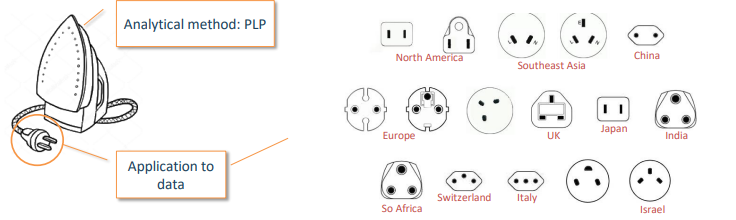
\includegraphics[width=0.60\textwidth]{figures/plancha1.png}
     %\caption{Ejemplo de la plancha con diferentes enchufes. Extraído de la web oficial \cite{OHDSIwebsite}}
    \label{fig:plancha1}
\end{figure}
\begin{figure}[H]
    \centering
    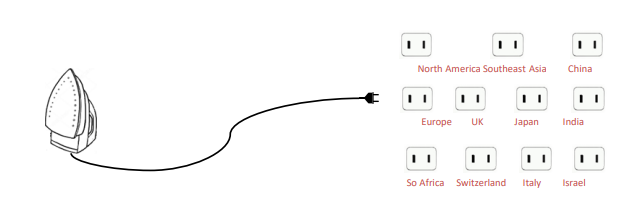
\includegraphics[width=0.70\textwidth]{figures/plancha2.png}
     \caption{Ejemplo de la plancha. Extraído de la web oficial \cite{OHDSIwebsite}}
    \label{fig:plancha2}
\end{figure}

    Como se muestra en la Figura \ref{fig:plancha2} ''Ejemplo de la plancha'', la plancha sería el diseño de un estudio observacional y el enchufe de pared, la base de datos. En el dibujo de arriba se presenta la problemática actual: un mismo estudio no se puede realizar o ''enchufar'' a distintas bases de datos porque no comparten la misma estructura. El objetivo de la organización se muestra abajo: estandarizar las bases de datos con una misma estructura para que un mismo estudio pueda aplicarse a diferentes bases de datos.

    Con este fin OHDSI promueve el uso del Modelo de Datos Común de OMOP (véase en mayor extensión en \ref{subsec:07cdm} ''Modelo de Datos Común'') para estandarizar las bases de datos observacionales. Por otro lado, para conducir los diferentes estudios de forma estandarizada, con el objetivo de fomentar su trazabilidad y reproducibilidad, se ofrecen marcos e instrucciones teóricas sobre cómo conducir los estudios (véase a continuación \ref{sec:05Evidencia} ''¿Cómo generar evidencia?'') y herramientas de análisis estandarizadas, como es el caso de ATLAS y otras herramientas (vease en mayor extensión en \ref{sec:07herramientas} ''Herramientas''). 
    
    Por tanto, \textbf{OHDSI se trata de un ecosistema de herramientas y estándares de salud.} Este ecosistema se describe en mayor detalle en el capítulo \ref{cap:07entorno} ''Entorno de Trabajo''.

    \item \textbf{Extracción de evidencia a partir de datos observacionales}. Es importante destacar que la finalidad de OHDSI no es solo recopilar y almacenar la información clínica de forma estándar, sino también la extracción de información o evidencia de la misma. 
    %La organización identifica la dificultad de extraer información trascendental de los datos clíncos debido a sus distintas morfologías y estructuras en las que son recogidos. 
    %Este es el propósito final y enfrenta muchos desafíos debido a la disparidad de los datos y técnicas de análisis. 
    
    El proceso de extracción de evidencia no es sencillo, como se muestra en la Figura \ref{fig:drawinJourney} ''Dibujo del proceso de extracción de evidencia'', y parte en un extremo de las diferentes bases de datos del mundo real (RWD) hacia la obtención fiable de evidencia del mundo real (RWE). %Por suerte, la organización también proporciona un conjunto de herramientas (véase \ref{sec:05herramientas} ''Herramientas'') para realizar más sencillamente todo el recorrido.

\begin{figure}[H]
    \centering
    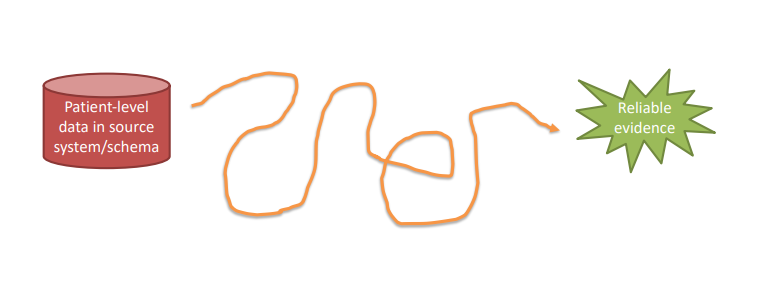
\includegraphics[width=0.80\textwidth]{figures/drawinJourney.png}
     \caption{Dibujo del proceso de extracción de evidencia. Extraído de la web oficial \cite{OHDSIwebsite}}
    \label{fig:drawinJourney}
\end{figure}

    \textbf{La organización se compromete fielmente con este cometido de facilitar la extracción de evidencia a partir de datos observacionales} y para facilitar este proceso ofrece de forma abierta todos los estándares y herramientas mencionados anteriormente. Esta es idea es fundamental en OHDSI y se describe en mayor detalle a continuación, en la sección \ref{sec:05Evidencia} ''¿Cómo generar evidencia?''.

\end{itemize}

%\section{Historia: Observational Medical Outcomes Partnership (OMOP)}

\section{¿Qué es OMOP?} \label{sec:05omop}

Es común encontrar en internet los términos OHDSI y \textbf{OMOP (Observational Medical Outcomes Partnership)}, utilizados de forma casi indistintiva. Si bien es verdad que OMOP se suele asociar mayoritariamente al CDM (\textit{Common Data Model}) también OHDSI mantiene gran relación con este modelo común de datos. Entonces, ¿cuál es la relación entre estas dos entidades? Pues bien, \textbf{la relación que guardan estas dos entidades es filial, OHDSI (2014-Actualidad) es la sucesora de OMOP (2008-2013)}.

OMOP nació en 2008 como una asociación público-privada presidida por la Administración de Alimentos y Medicamentos de EE. UU. y administrada por la Fundación de los Institutos Nacionales de Salud y financiado por un consorcio de compañías farmacéuticas en colaboración con otros investigadores académicos y socios de datos de salud \cite{stang2010advancing}. El propósito inicial de OMOP fue impulsar la ciencia de la vigilancia activa de la seguridad de los productos médicos mediante el análisis de datos observacionales de atención médica \cite{stang2010advancing}. Sin embargo, durante su desarrollo, se enfrentó a los desafíos técnicos de llevar a cabo investigaciones en bases de datos observacionales muy heterogéneas entre sí.

Frente a esta problemática, el resultado fue el desarrollo de un Modelo Común de Datos (CDM) como un mecanismo para estandarizar la estructura, el contenido y la semántica de los datos observacionales %y hacer posible escribir código de análisis estadístico que fuera reutilizable para estudios en distintas fuentes de datos 
\cite{overhage2012validation}. Los experimentos de OMOP demostraron la viabilidad de establecer un CDM que además reuniese diferentes vocabularios estandarizados, reuniendo en un mismo estándar diversos tipos de datos de diferentes entornos de atención y representados por diferentes vocabularios de origen. Esta característica facilitó la colaboración y aumentó el interés entre diferentes instituciones lo que promovió o un enfoque de ciencia abierta \cite{OHDSIbook}. OMOP puso todo su trabajo a disposición del público, incluidos diseños de estudio, estándares de datos, código de análisis y hallazgos empíricos, para mejorar la transparencia y fomentar la confianza en su investigación. 

Al término del proyecto, el Modelo Común de Datos (CDM) de OMOP había evolucionado hasta respaldar un abanico  amplísimo de aplicaciones analíticas de todo el sistema de salud, no solo de la industria farmacéutica. Finalmente, el equipo de investigación acordó que el fin de dicho proyecto debía ser el origen de uno nuevo y a partir de esta idea nació OHDSI \cite{OHDSIbook}.


\section{¿Cómo generar evidencia?} \label{sec:05Evidencia}

La extracción de evidencia a partir de estudios de datos clínicos observacionales es la finalidad fundamental de OHDSI (véase \ref{sec:05OHDSI} ''¿Qué es OHDSI?''). 

%Este proceso generalmente es bastante complejo, debido a la disparidad de estructuras en la que se recopilan los datos de salud y la disparidad de metodologías en las que se conducen los estudios, lo que imposibilita y/o dificulta la interoperabilidad entre los sistemas de información sanitaria (véase \ref{sec:01Contexto} ''Contexto'').

%Frente a ello, OHDSI propone un marco estándar para generar evidencia basada en la estandarización de los datos clínicos al Modelo de Datos Común de OMOP y la definición de tres tipos de estudios observacionales o ''\textit{casos de uso}''. Además proporciona un conjunto de herramientas estandarizadas con las que realizar todas las tareas implicadas en el proceso con el fin de facilitar la generación de evidencia interoperable entre los distintos nodos y organizaciones de su comunidad.

Por ello, no es casualidad que la invitación que hace OHDSI a sus colaboradores lleve el slogan \textit{''Join the Journey''} (véase anteriormente \ref{subsec:05caracteristicas} ''Características de la organización''), sino que es un guiño al propósito al que se unen: al camino desde los datos hacia la evidencia o, en ingles, \textit{\textbf{"The Journey from data to evidence"}}.  

%A continuación, en las secciones \ref{subsec:05journey}, \ref{subsec:05invest}, \ref{subsec:05vias} se presentan los conceptos fundamentales para comprender este proceso desde el punto de vista de la organización.

%\subsection{El camino desde los datos hacia la evidencia} \label{subsec:05journey}

\begin{figure}[H]
    \centering
    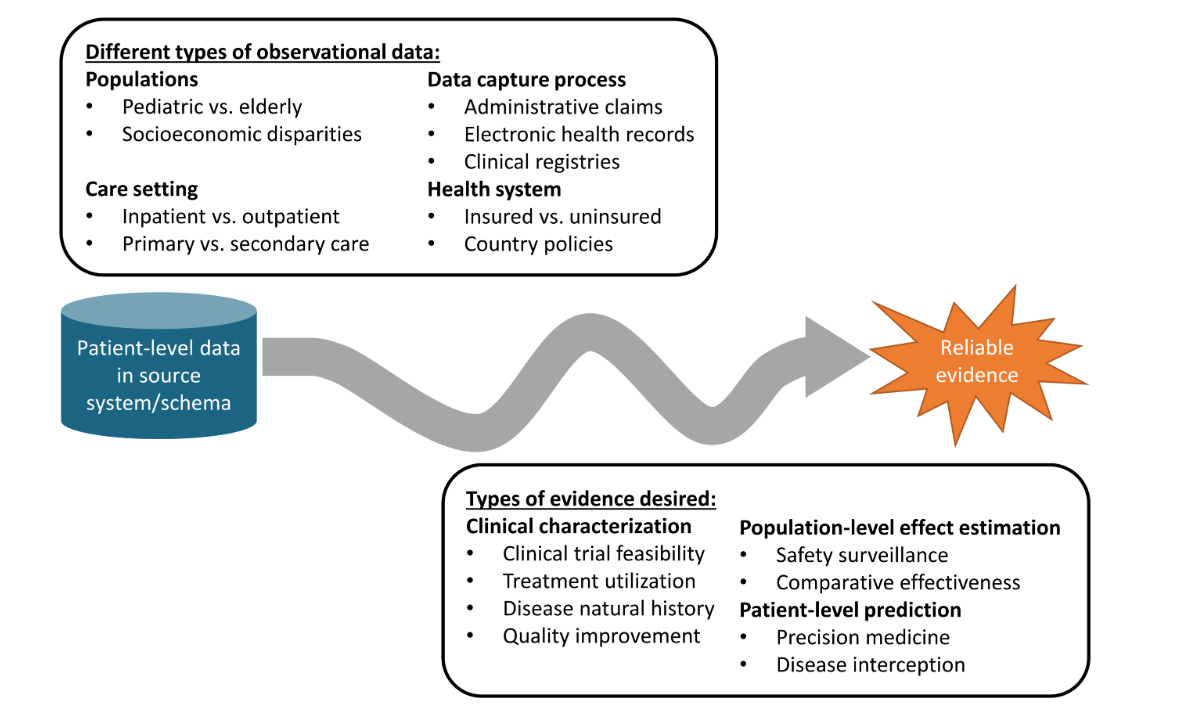
\includegraphics[width=0.80\textwidth]{figures/journeyDataToEvidence.png}
     \caption{\textit{The Journey from Data to Evidence}. Extraído del Libro de OHDSI \cite{OHDSIbook}}
    \label{fig:journeyDataToEvidence}
\end{figure}

La Figura \ref{fig:journeyDataToEvidence} ''The Journey from Data to Evidence'' complementa a la anterior Figura \ref{fig:drawinJourney} ''Dibujo del proceso de extracción de evidencia'' añadiendo mayor información en los extremos del recorrido, definiendo cuatro tipos distintos de bases de datos observacionales y tres tipos de evidencia que se quiere generar: la caracterización clínica \textit{(clinical characterization)}, la estimación de efectos a nivel de población (\textit{Population-level effect estimation)} y la predicción a nivel de paciente \textit{(Patient-level prediciton)}. Estos tres ''casos de uso'' se presentan en mayor profundidad a continuación en  \ref{subsec:05casosUso} ''Casos de uso para la investigación''.

%Esta definición de tres \textit{''casos de uso''} en la investigación se detalla en mayor profundidad en

Con ello la organización define un marco para llevar a cabo \textbf{estudios observacionales o fenotípicos} sobre datos. Un estudio observacional es una investigación que observa y recopila información sobre individuos o fenómenos sin intervenir en ellos.
En el caso del estudio sobre datos, en vez de realizar seguimientos de estudios clínicos en vivo, se simulan estos estudios sobre una base de datos. Cuando la evidencia se extrae sobre datos del mundo real (\textit{RWD}), se denomina evidencia del mundo real (\textit{Real World Evidence, RWE}). 

En OHDSI la conducción de estos estudios observacionales se realiza mediante el diseño y estudio de cohortes en la base de datos. Concretamente, se trata de \textbf{estudios de cohortes retrospectivos} porque los sujetos se estudian después de haberse producido la enfermedad, utilizando para ello bases de datos que tengan registrada información histórica de la enfermedad y de los factores de riesgo que hayan podido provocar dicha enfermedad.

A continuación en \ref{subsec:05cohortes} ''Cohortes'' se presenta este concepto en profundidad.

%Frente a la disparidad de los datos y la finalidad con la que son recogidos, OHDSI presenta el Modelo de Datos Común (véase la subsección \ref{subsec:05cdm} ''Modelo de Datos Común'') y para la extracción de evidencia, la investigación metodológica mediante tres casos de uso fundamentales: la caracterización clínica de una cohorte, la estimación a nivel de población y la predicción a nivel de paciente (véase subsección \ref{subsec:05investMetodolog} ''Investigación metodológica'').

%De esta forma, OHDSI promueve una vía para generar evidencia interoperable entre las distintas organizaciones que interactúan a través de su red mundial, dicho de otra forma, da soporte para que diferentes estudios se realicen siguiendo una misma metodología que facilite su comprensión y reproducibilidad de forma global, como se sugería en el ejemplo de la plancha (véase anteriormente \ref{subsec:05caracteristicas} ''Características de la organización'').

\subsection{Cohortes} \label{subsec:05cohortes}

%Además, una característica fundamental de las investigaciones que se llevan acabo en OHDSI es que giran entorno al paciente, que es además el núcleo central del Modelo de Datos Común de OMOP. 

El componente central de cualquier investigación en OHDSI es el paciente, del que se recopilan las denominadas ''historias del paciente''. \textbf{Para cada evento clínico que sucede se recoge una historia del paciente o \textit{Patient Journey}}. %Es importante no confundir este concepto con la Historia Clínica Electrónica de un paciente (HCE) que recoge una ficha con todos los eventos que han le sucedido a lo largo de su vida. 
Las investigaciones observacionales se diseñan para extraer información sobre la recopilación de todas las historias de paciente registradas en la base de datos.

La historia del paciente,  como se muestra en la Figura \ref{fig:patientJourney} ''The patient journey'', es por tanto, una ventana temporal que recoge un evento clínico que le sucede a un paciente en un período de tiempo concreto. El evento se describe mediante tres períodos de tiempo: la enfermedad (rojo), el tratamiento (naranja) y el efecto (verde); y a partir de distintas características como enfermedades (\textit{conditions}), medicamentos (\textit{drugs}), procedimientos (\textit{procedures}) y pruebas (\textit{measurements}).

\begin{figure}[H]
    \centering
    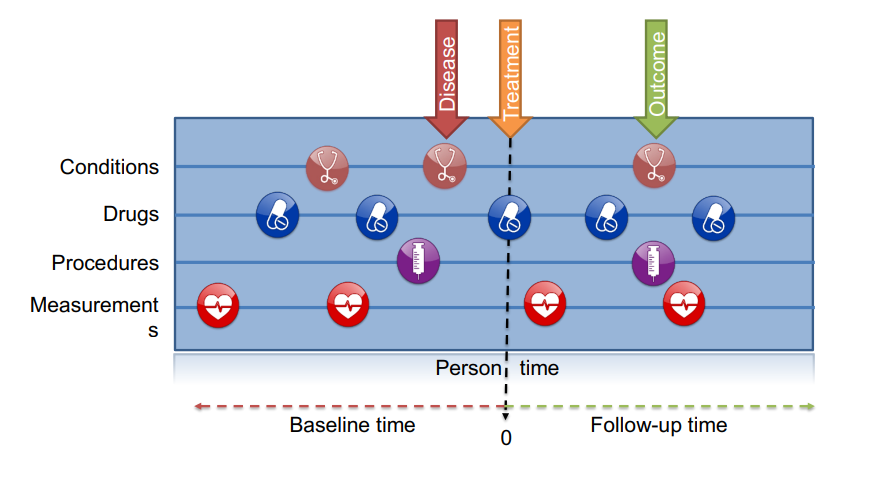
\includegraphics[width=0.80\textwidth]{figures/patientJourney.png}
     \caption{\textit{The patient journey}. Extraído de la página web oficial \cite{OHDSIbook}}
    \label{fig:patientJourney}
\end{figure}

Los pacientes se pueden agrupar en \textbf{cohortes} cuando comparten historias y características similares, al igual que a la hora de realizar un estudio clínico en vivo. Las diferentes  prácticas para los análisis de cohortes darán lugar a los diferentes tipos de evidencia deseada (caracterización, estimación a nivel de población, predicción a nivel de paciente). \textbf{Por tanto, el componente central para generar evidencia en OHDSI es el diseño de cohortes.}

%\begin{figure}[H]
%\centering
%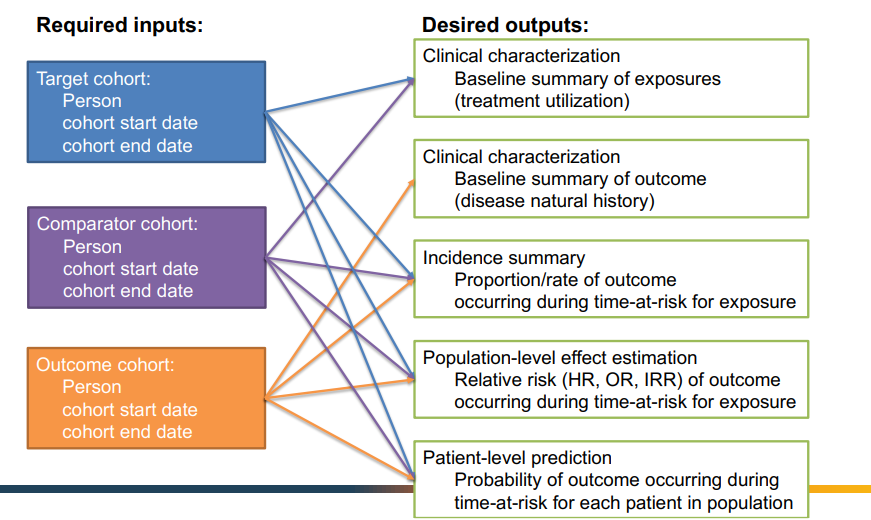
\includegraphics[width=0.70\textwidth]{figures/studyIO.png}
%     \caption{La definición de cohortes es el componente esencial para la generación de evidencia. Extraído del Tutorial2022 publicado en la web oficial \cite{OHDSIwebsite}}
%    \label{fig:studyIO}
%\end{figure}

\textbf{En OHDSI una cohorte es un ''conjunto de personas que satisface uno o más criterios de inclusión durante un periodo de tiempo concreto''} \cite{OHDSIbook}. Definir correctamente la cohorte es fundamental a la hora de realizar cualquier estudio fenotípico en OHDSI y es crucial para realizar un buen análisis \cite{hripcsak2018high}. A continuación se presenta esquemáticamente la estructura fundamental de una cohorte, denominada en OHDSI ''anatomía de una cohorte''.

\begin{figure}[H]
\centering
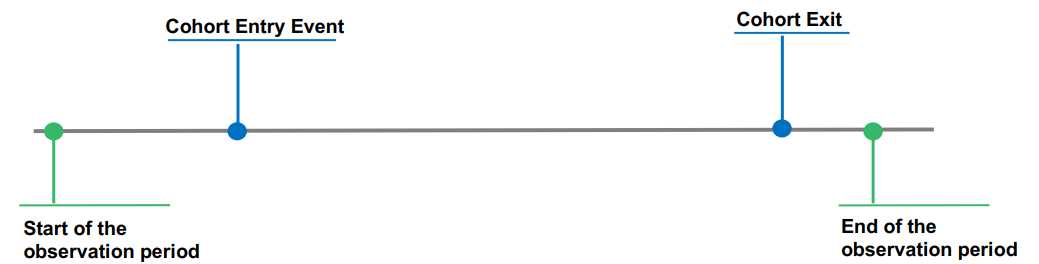
\includegraphics[width=0.90\textwidth]{figures/cohortAnatomy.png}
     \caption{''Anatomía de una cohorte''. Extraída del Tutorial 2022 publicado en la web oficial \cite{OHDSIwebsite}}
    \label{fig:cohortAnatomy}
\end{figure}

La investigación observacional comprende un intervalo temporal delimitado por el comienzo del período de  observación (\textit{Start of the observation period}, en verde) y el fin del periodo de observación (\textit{End of the observation period}, en verde).

Dentro del periodo de observación, la cohorte se define con un  evento de entrada a la cohorte (\textit{Cohort Entry Even}t, en azul) y un evento de salida de la cohorte (\textit{Cohort Exit}, en azul). 

\begin{itemize}

    \item \textbf{Evento de entrada.} Define el evento que cualifica al paciente para entrar a la cohorte. El conjunto de pacientes que satisfacen el evento de entrada conforman la cohorte inicial. 

    \item \textbf{Evento de salida.} Define el evento de salida de la cohorte, cuando el paciente ya no es elegible para formar parte de la cohorte.

\end{itemize}

Adicionalmente, la cohorte puede definirse más específicamente mediante una serie de \textbf{criterios de inclusión}. La cohorte que satisface todos los criterios de inclusión se denomina cohorte cualificada. La elección de los criterios de inclusión de la cohorte es fundamental en el diseño del estudio observaciona.

La terminología que se emplea para describir los eventos clínicos que definen la cohorte se debe agrupar en grupos de conceptos. \textbf{En OHDSI, los grupos de conceptos son expresiones reusables que representan un listado de conceptos pertenecientes al Vocabulario que definen un evento clínico concreto}.  Son el equivalente a las ''listas de códigos'' que se utilizan en los estudios observacionales \cite{OHDSIbook}.

\subsection{Casos de uso para la investigación} \label{subsec:05casosUso}

Con el fin de estandarizar y proveer un marco metodológico en el camino hacia la generación de evidencia, OHDSI define tres casos de usos que establecen los diferentes tipos de estudio que se pueden realizar: (i) la caracterización, (ii) la estimación a nivel de población (iii) la predicción a nivel de paciente.

\begin{figure}[H]
\centering
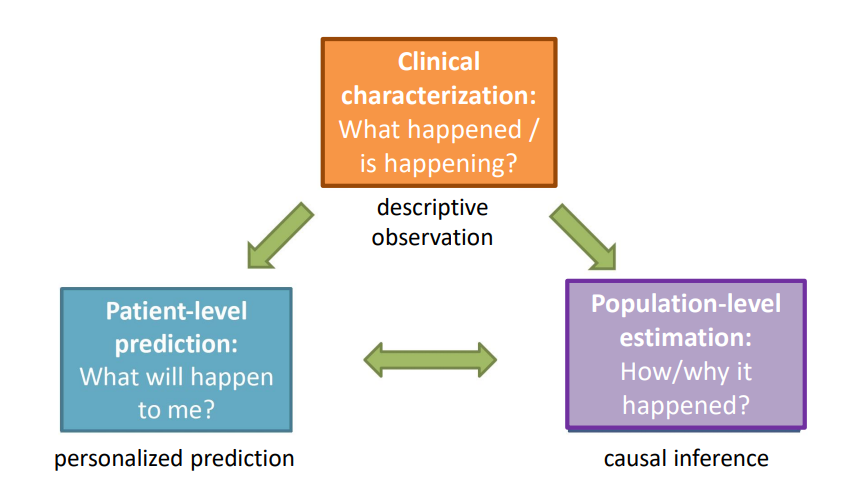
\includegraphics[width=0.80\textwidth]{figures/useCases.png}
     \caption{Esquema simplificado de los casos de uso para la investigación en OHDSI. Extraído del Symposium 2023, publicado en la web oficial \cite{OHDSIwebsite}}
    \label{fig:useCases}
\end{figure}

%Estos tres casos de uso se presentan generalmente en los \textit{Symposium} y \textit{Workshops}, para dar a conocer a la comunidad el esquema propio de investigación de OHDSI. Además el Libro de OHDSI \cite{OHDSIbook} los presenta de forma general en el capítulo 7 y de forma específica para cada caso de uso en los capítulos 11, 12 y 13, respectivamente. 

Anteriormente se definieron las historias de paciente como marco fundamental de la investigación (véase \ref{subsec:05cohortes} ''Cohortes''). Cada caso de uso extrae un tipo de evidencia distinto a partir de la historia del paciente, tal y como se muestra a continuación en la Figura \ref{fig:useCasesJourney} ''Esquema de los casos de uso encuadrado en la historia del paciente''.


\begin{figure}[H]
\centering
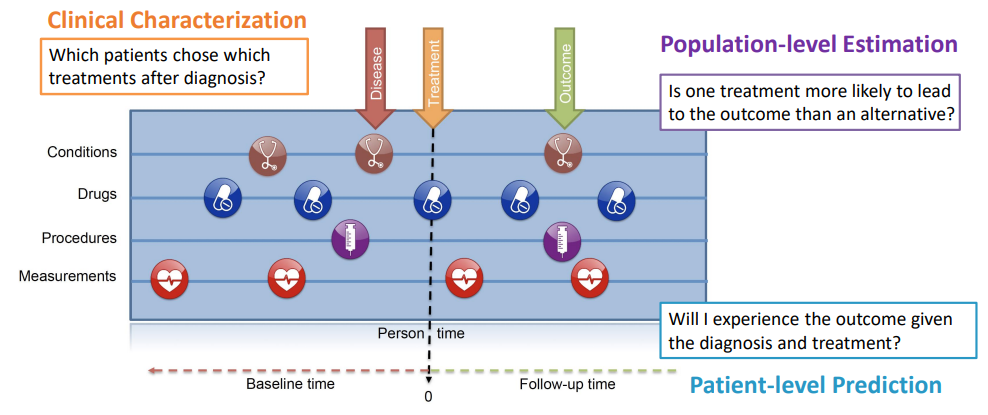
\includegraphics[width=1\textwidth]{figures/useCasesJourney.png}
     \caption{Esquema de los casos de uso encuadrado en la historia del paciente. Extraído del Symposium 2023 publicado en la web oficial \cite{OHDSIwebsite}}
    \label{fig:useCasesJourney}
\end{figure}

La historia del paciente definirá la pertenencia o no del paciente a una cohorte y sobre esa cohorte se realizarán los distintos tipos de estudio. \textbf{El conjunto de estos tres casos de uso y la definición de cohortes conforma la metodología OHDSI para la generación de evidencia}. A continuación se describe brevemente cada uno de los casos de uso. 

\subsubsection{Caracterización}

La caracterización busca la caracterización a nivel estadístico de una cohorte o una base de datos. Es una mera descripción estadística de los datos, sin realizar inferencias, predicciones o análisis más complejos, simplemente observando la base de datos.

Responde a la pregunta de investigación: \textbf{¿Qué les ha pasado?}

Obtiene como resultados: recuentos y porcentajes, medias, estadísticas descriptivas, ratios de incidencia...

\subsubsection{Estimación a nivel de población}

La estimación a nivel de población busca realizar inferencias causales sobre los efectos de las intervenciones sanitarias en la población. Se pretende entender los efectos causales para comprender las consecuencias de las acciones.

Responde a la pregunta de investigación: \textbf{¿Cuáles son los efectos causales?}

Obtiene como resultados: riesgos relativos, efectos causales, correlación entre variables, comparaciones de efectividad, asociaciones…

\subsubsection{Predicción a nivel de paciente}

La predicción a nivel de paciente busca, en base a los datos obtenidos de los conjuntos de pacientes en la base de datos, realizar predicciones concretas para individuos concreto.

Responde a la pregunta: \textbf{¿Qué me pasará a mi como paciente?}

Obtiene como resultados: probabilidades para un individuo, fenotipos probables, grupos de riesgo… 


\subsection{Vías de implementación del análisis} \label{subsec:05vias}

Para realizar un análisis, OHDSI distingue tres vías alternativas para generar la evidencia a partir de la base de datos estandarizada al OMOP CDM. Estas tres alternativas se muestran a continuación en la Figura \ref{fig:analysisImplementations} ''Tres vías para la implementación de un análisis observacional'', extraída del capítulo 8 del Libro de OHDSI.

\begin{figure}[H]
    \centering
    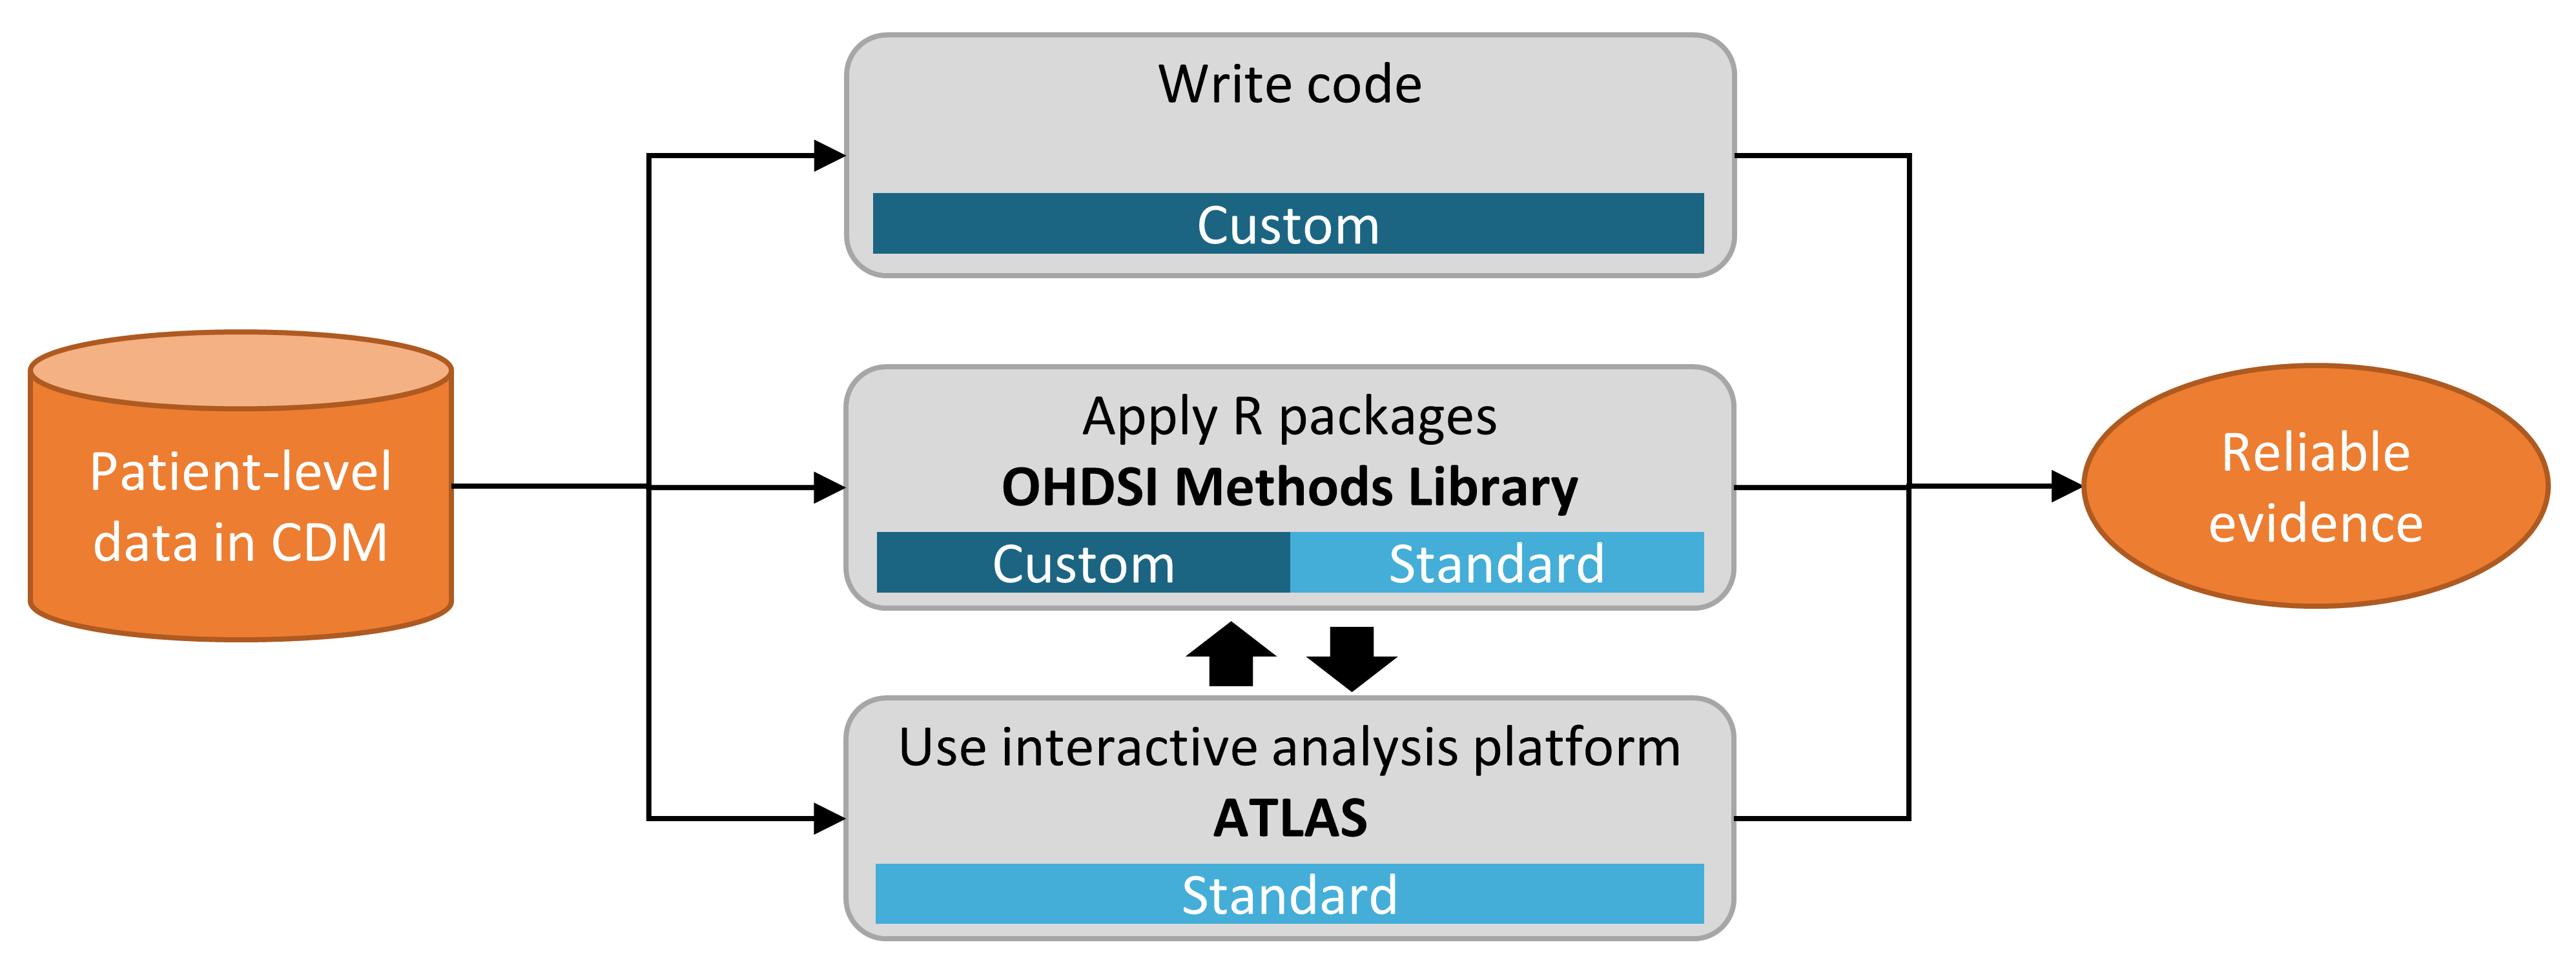
\includegraphics[width=0.80\textwidth]{figures/analysisImplementations.png}
     \caption{Tres vías para la implementación de un análisis observacional. Extraído del Libro de OHDSI \cite{OHDSIbook}}
    \label{fig:analysisImplementations}
\end{figure}

Cada vía se evalúa en cuanto a lo personalizada (\textit{custom}) o estandarizada (\textit{standard}) que es. A estas alturas se debe conocer que la vía más recomendada para implementar el análisis será la más estandarizada, es decir, la tercera vía.

La problemática que presentan la primera y la segunda vía consiste en ser en mayor o menor medida vías customizada, lo que genera problemas de interoperabilidad y reproducibilidad de los estudios. Si bien la primera vía consiste en la programación directa de código para realizar las consultas  (no hay ningún tipo de estandarización, distintos lenguajes de programación, funciones personalizadas) al menos la segunda vía hace uso de librerías estándares en R que OHDSI ofrece (\textit{OHDSI Methods Library}) pero, aunque se use el mismo lenguage de programación y funciones, los scripts pueden ser tan distintos que aún dificulten la interoperabilidad.

Por tanto, la tercera vía se presenta como la alternativa óptima por ser la más estandarizada y es la que empleará el TFG en el estudio práctico. Esto es, usar la herramienta interactiva \textit{low-code} de análisis de datos que ofrece OHDSI, denominada \textbf{ATLAS}, sin necesidad de programar directamente código.

\section{Conclusiones} \label{sec:05conclusion}

En este capítulo se recogen las características fundamentales de OHDSI con el fin de comprender la relevancia de la organización en el panorama sanitario, como sucesora de OMOP y gran candidata para subsanar las dificultades en términos de interoperabilidad y estandarización de la investigación observacional.

Además se explora en mayor profundidad la metodología que promueve la organización en cuanto a la generación de evidencia clínica, a partir del concepto de cohorte y los estudios de caracterización, estimación a nivel de población y estimación a nivel de paciente.